% !TeX root = ../index.tex

\section{Introduction}\label{sec:introduction}

\citeauthor{boner_reactive_2014} in their \citetitle{boner_reactive_2014} outline qualities of modern \glspl[]{is} that make them better to use as well as easier to develop, maintain and extend.
They summarize these qualities under the term \emph{reactive}.

In my work at SAP~SE, my team and I are building \gls[]{saas} business applications that are supposed to offer a great user experience, while being as cost-effective as possible to develop, operate, maintain and extend.
As a part of that effort we aim to make our product reactive by applying the microservice pattern and using asynchronous, message-driven integration.
While applying these design paradigms to the implementation of business features we sometimes encounter situations where the feature requires synchronous communication between two microservices.

This requirement confronts us with a non-trivial design decision of how to best implement it in our system architecture that is dominated by asynchronous integration.
Various works in the professional literature examine the problem briefly but the solution approaches which they offer do not go into great detail \parencites[706--708]{millett_patterns_2015}[30--32]{stopford_designing_2018}[87--89]{richardson_microservices_2019}.
In academics, this particular problem has received no consideration so far.

The goal of this work is to create a generic concept for implementing synchronous communication in a reactive \gls[]{is}.
Such a concept addresses a problem that is not only immediately relevant to my organization but is also transferable to various other \gls[]{is} architectures, since the use of the microservice pattern and message-driven integration is widespread.
Furthermore, this work adds to the knowledge base by clearly examining the problem space, discussing the solution approaches in the professional literature and constructing a new concept for addressing it.

To that end, the work applies the \gls[]{dsr} process outlined in \cite{alturki_design_2011} which is discussed in more detail in the following section \ref{sec:method}.
Afterwards, section \ref{sec:foundations} establishes necessary theoretical foundations and is followed by section \ref{sec:problem} which examines the problem space in greater detail before section \ref{sec:concept} derives a concept to address the problem.
% , which is then evaluated in section \ref{sec:evaluation}.
Lastly, section \ref{sec:conclusion} discusses the results and concludes with an outlook on further work.

\clearpage
\section{Methodology}\label{sec:method}

The goal of this work places it firmly in the domain of \gls[]{dsr}.
Various researchers have constructed formalized methods for conducting \gls[]{dsr} as is presented in \cite[]{dresch_design_2015}.
This work follows the research method that is synthesized in \cite[]{alturki_design_2011} because it is both comprehensive and practical.
The rest of this section discusses the method in greater detail and how this work makes use of it.

The first two steps in \citeauthor{alturki_design_2011}'s roadmap are to \enquote{Document the Spark of an Idea/Problem} and to \enquote{Investigate and Evaluate the Importance of the Problem/Idea} \parencite[110--111]{alturki_design_2011}.
Section \ref{sec:introduction} has already introduced the problem and discussed its relevance.
Further examination of the problem is taken up in section \ref{sec:problem} which then also evaluates the feasibility of a new solution.
The next step on the roadmap \parencite[111]{alturki_design_2011}.

Furthermore, section \ref{sec:problem} together with the research goal defined in section \ref{sec:introduction} define the research scope and resolve that the problem falls within the domain of design science, more specifically, \gls[]{dsr}.
Thereby it completes the next three steps on the roadmap \parencite[111]{alturki_design_2011}.
The theme of the research conducted here is the construction of an artifact and excludes its evaluation so that the scope intended for this work is not exceeded.\todo{maybe mention artificial evaluation}
This addresses the seventh step on the roadmap: \enquote{Resolve Theme} \parencite[114]{alturki_design_2011}.

The next five steps on the roadmap are addressed in section \ref{sec:concept}: \enquote{Define Requirements}, \enquote{Define Alternative Solutions}, \enquote{Explorer [\emph{sic}] Knowledge Base Support of Alternatives}, \enquote{Prepare for Design and/or Evaluation} and \enquote{Develop} \Parencite[114--115]{alturki_design_2011}.
The step \enquote{Evaluate} is delegated to further work and the last step \enquote{Communicate findings} is addressed implicitly by this work \Parencite[115--116]{alturki_design_2011}.

\clearpage
\section{Foundations}\label{sec:foundations}

This section introduces concepts that are required as a foundation for the discussion in the following sections.
First, the qualities of reactive \gls[]{is} as defined by \cite[]{boner_reactive_2014} are presented followed by an overview of the microservice design pattern and message-based integration---two design approaches commonly used to design reactive \gls[]{is}.

\subsection{Reactive Information Systems}

In \cite[]{boner_reactive_2014} the authors define four qualities that they observed in various modern \glspl[]{is} of different domains.
They describe how these qualities combine to make an \gls[]{is} what they call \emph{reactive} and how a reactive systems are more flexible, scalable, changeable and offer a superior user experience.

\begin{figure}[h]
  \centering
  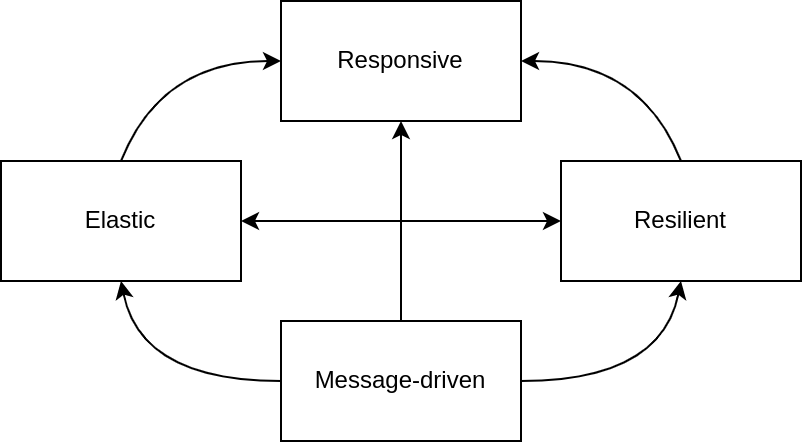
\includegraphics[width=0.9\textwidth]{reactive.drawio.png}
  \\\emph{Source}: \cite[]{boner_reactive_2014}
  \caption{The Qualities of a Reactive Information System}\label{fig:reactive}
\end{figure}

Figure \ref{fig:reactive} shows the four qualities of a reactive system and how they relate to each other.
Most importantly, a reactive system is \emph{responsive}.
That means the system provides its service in a consistent quality with consistent, rapid response times.

Furthermore, a reactive system must be \emph{resilient}.
It must remain responsive even if it faces partial failure.
The system is composed of isolated components that can fail and recover without bringing down the system as a whole.
This composition is transparent for the client.

No less important that resilience is being \emph{elastic}.
A system must remain responsive under varying workload.
Its components can be scaled up or down according to demand to achieve elasticity in the most cost-effective manner.
Both elasticity and resilience require the system's composition of isolated components.

Lastly, the fundamental quality of a reactive system is being \emph{message-driven}.
They integrate their components by implementing a mechanism of asynchronous message-passing.
Asynchronous, non-blocking communication decouples the components both functionally and temporally.
Thereby it allows for them to be more isolated and by extension makes the system more resilient and elastic.

\subsection{Microservice Architecture}

This common architectural style is an approach to designing an application as a suite of small, loosely-coupled services.
Each service runs in its own process and is independently deployable.
They communicate amongst each other via lightweight mechanisms, such as HTTP APIs or asynchronous message-passing.
\parencite{fowler_microservices_2014}

Microservices are structured around business capability rather than technical function.
This means that instead of having a team of \gls[]{ui} experts work on the entire \gls[]{ui} of the application, a team of middleware specialists work on all the middleware and a team of all data base specialist work on all the data base administration, the teams are organized in a cross-functional manner around certain business capabilities.
\parencite{fowler_microservices_2014}

When looking at how to decompose the application domain into distinct business capabilities, \gls[]{ddd} is commonly used.
Among other things, it offers various patterns for mapping and understanding problem domains as well as for dissecting them into smaller, more controllable sub-domains.
The approach encourages domain experts and developers to create a common language, to create models of relevant sub-domains as a basis for development and to clearly separate them from other sub-domains.
\gls[]{ddd} is an approach to building software for complex problem domains \parencite[4--14]{millett_patterns_2015}.

These sub-domains with their models, terminology and context are referred to as bounded contexts \parencite[79--85]{millett_patterns_2015}.
In the development of microservices, these bounded contexts are commonly used as a basis for structuring the suite of services.

The the microservice pattern offers the decomposition of a system into isolated components required for a reactive system to be resilient and reactive.
Together with message-based integration it can serve as the conceptual foundation for reactive \glspl{is}.

\subsection{Message-driven Integration}

The foundational quality of a reactive \gls[]{is} is being message-driven.
System architectures commonly employ a dedicated software components solely for that purpose---the so-called \gls[]{mom}.
\gls[]{mom} act as dedicated glue-ware that facilitates asynchronous message-passing between other software components.
The software offers publish/subscribe functionality for packets of data called messages.
Clients act as either \emph{publishers} or \emph{consumers}, or as both simultaneously.
Publishers connect to the \gls[]{mom} to address a message to a specific communication channel often referred to as a \emph{topic}.
Consumers subscribe themselves to one or multiple topics and receive all messages that are published to them from the \gls[]{mom} via either a push- or pull-mechanism.
\parencite{banavar_case_1999}

Other names that might be used for \gls[]{mom} are \emph{message bus} or \emph{message broker}.
Depending on the source, these terms might be used synonymously or to refer to different variants of \gls[]{mom}.
Furthermore, some \gls[]{mom} concepts and implementations can have routing and transformation functionality for messages as part of the component.
\cite{banavar_case_1999} for example write of \enquote{message flow graphs} as part of \gls[]{mom} to offer this functionality.
The text below however uses the term message broker and means it to be a simple \gls[]{mom} as described in the previous paragraph.

\clearpage
\section{A Message-Driven Information System}\label{sec:problem}

This section examines the hypothetical architecture design of a reactive \gls[]{is} that implements a common business process to explore the problem of synchronous communication in message-driven systems.
To begin, the following introduces the business process which is implemented by the \gls[]{is}---the \gls[]{p2p} process.
The process relatively simple and common to many organizations.
Therefore, it serves as a good example and does not distract from the technical discussion below.
After the \gls[]{p2p} process, the text introduces the sample architecture and uses it as a basis for the problem discussion.

\subsection{The Procure-to-Pay Process}

Figure \ref{fig:procure-to-pay} shows the distinct steps of the \gls{p2p} process.
Since it only serves as the background for technical discussion this representation of the process is intentionally simple.

On the \enquote{procure} side, the process begins with a request.
For example, when an employee of an organization requests a new stack of printing paper, they would create a request for it in the system.
After the request has been created, it requires the approval of a supervisor.
A cost center manager, for example.
Once the request is approved, the organization's purchasing department can create an order which is then sent to the supplier.

\begin{figure}[h]
  \centering
  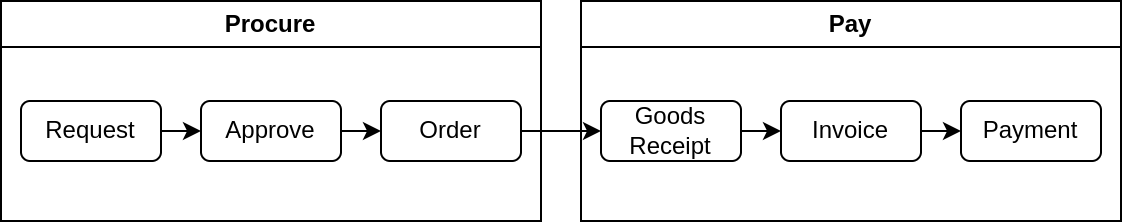
\includegraphics[width=0.9\textwidth]{procure-to-pay.drawio.png}
  \caption{The Procure-to-Pay Process}\label{fig:procure-to-pay}
\end{figure}

When the ordered goods are delivered to the organization, the process continues on the \emph{pay} side.
The goods are inspected and a goods receipt is created which is checked against the supplier's invoice.
If everything is in order, payment is made to the supplier.

The example architecture implementing this process is introduced below.
To keep it concise, it only implements the \emph{procure} part of the process.

\subsection{A Reactive Procurement Application}

Figure \ref{fig:example-architecture} shows the example architecture.
The procurement domain is decomposed into three bounded contexts: Request, Order and Workflow.
Each context is implemented by a dedicated microservice.

The \gls{ui} is fragmented into a set of web-applications accessed by users via their internet browsers.
These fragments are not strictly separated by bounded context, but rather by use case, with the aim of providing a superior user experience.
For example, purchasers may need to edit an employee's request to correct the description or price because the employee's initial inputs were insufficient.

The microservices communicate with each other by asynchronous message-passing via a message broker.
They consume and publish messages with domain events to and from domain-specific topics within the broker.

\begin{figure}[H]
  \centering
  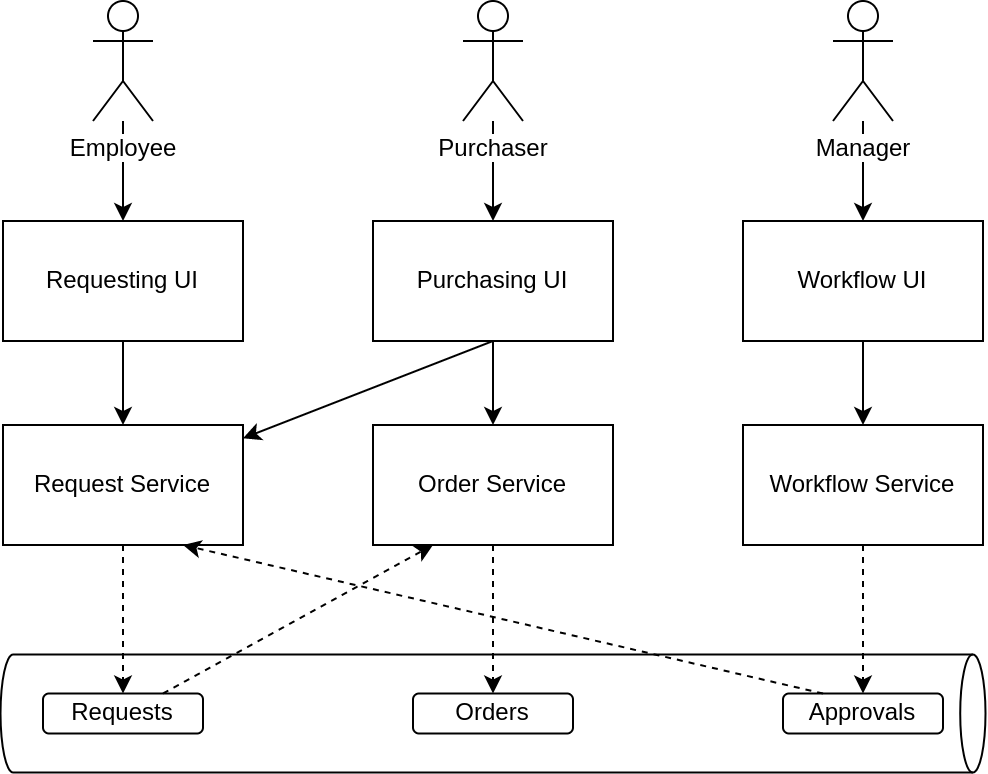
\includegraphics[width=0.9\textwidth]{architecture.drawio.png}
  \caption{The Example Architecture}\label{fig:example-architecture}
\end{figure}

In the figure, the different actors that use the \gls{is} in the context of the procurement process are shown at the top.
They interact with the system via the \gls{ui} fragments shown below as indicated by the arrows.
The fragments in turn interact with the microservices as indicated by the arrows.
Employees can request goods via the \emph{Requesting UI} and purchasers can edit requests as well as create orders via the \emph{Purchasing UI}.
Hence, the \emph{Purchasing UI} interacts with both the \emph{Request Service} and the \emph{Order Service}.
Requests are approved by managers via the \emph{Workflow UI} that interacts with the underlying \emph{Workflow Service}.
Although they are omitted in the diagram, each microservice is assumed to have a dedicated persistent storage.

The asynchronous communication of the microservices via the broker is represented in figure \ref{fig:example-architecture} by the dashed arrows.
The \emph{Request Service} publishes events to the \emph{Requests} topic.
These events---in sum---contain all the information on all requests that exist in the system.
Listing \ref{lst:request-created} shows what an event of the request domain may look like.

\begin{listing}[h]
  \inputminted{json}{assets/src/request-created.json}
  \caption{An example for a \texttt{RequestCreated} domain event}\label{lst:request-created}
\end{listing}

The \emph{Order Service} replicates the requests by aggregating the events from the \emph{Requests} topic.
When an order is created via the \emph{Order Service}, it publishes an appropriate event to the \emph{Orders} topic.
From there, it could theoretically be consumed by other \glspl{is} to, for example, send the order to suppliers via mail or e-mail, or to reserve a budget in the company's accounts.
Finally, the \emph{Workflow Service} publishes to the \emph{Approvals} topic when a manager approves a request.
The \emph{Request Service} consumes these events to update the status of a request when it has been approved.
This status change is then replicated to the \emph{Order Service} so that purchaser can create an order for the request.

\subsection{The Need for Synchronous Communication}

The system architecture above is missing a crucial part.
Namely, how the \emph{Workflow Service} is notified about new requests that need to be approved.
An easy way of achieving this would be for the \emph{Workflow Service} to also consume events from the \emph{Requests} topic.
In this way it would be notified when new requests are created and need to be approved.

While that is a simple solution, it is also cumbersome to extend.
This becomes clear considering this hypothetical future requirement: Orders require a final approval before they are sent out to the supplier.
To address this requirement, the \emph{Workflow Service} would need to listen to the \emph{Orders} topic as well.
The same would be true for any other domain entity that might require approvals in the future.

Instead of the \emph{Workflow Service} picking up the required approvals from the other bounded contexts, the scheme can be inverted so that the bounded contexts tell the service when they require an approval.
This could be implemented by adding new topic \emph{Approval Requests} to the message broker and letting each domain that requires approvals publish events to it.
The \emph{Workflow Service} would consume and offer the approval requests to the appropriate users and publish events with the users' decisions to the \emph{Approvals} topic as it already does.
In this setup, the \emph{Workflow Service} and other bounded contexts fall into the traditional roles of server and clients.

The solution however is still missing an aspect.
Clients of the \emph{Workflow Service} need to know whether the service has received the approval request for a particular entity and whether it was properly processed.
They require this information to prevent approval requests being lost if, for example, due to a bug in the \emph{Workflow Service} it cannot process a couple of messages and drops them instead.
With the appropriate feedback, the other microservices could re-send the request after a waiting period to ensure that it is processed.
It furthermore enables them to provide accurate feedback to their users.
At this point the required mode mode of communication is synchronous because the clients need a reply from the server within a certain time frame.

A simple solution to this problem is to break with the message-driven paradigm and let the other bounded contexts use an inherently synchronous communication pattern (like HTTP) to tell the \emph{Workflow Service} about new approval requests.
This approach, however, has its downsides and the problem lies in choosing the best solution.

Regarding the research roadmap of \cite[]{alturki_design_2011}, this section has documented the problem space and demonstrated the feasibility of a solution.
As described in section \ref{sec:method}, the following section continues the roadmap and explores the solution space.

\clearpage
\section{Concept}\label{sec:concept}

% \clearpage
% \section{Evaluation}\label{sec:evaluation}

\clearpage
\section{Conclusion}\label{sec:conclusion}
